Для реализации узла были использованы следующие примитивы из библиотеки САПР Quartus II:
\begin{itemize}
\item элемент <<НЕ>>
\item элемент <<6-И>>
\item элемент <<2-И>>
\item элемент <<2-ИЛИ>>
\end{itemize}
Из настраиваемых компонентов библиотеки САПР Quartus II использовались следующие:
\begin{description}
\item[5-разрядный счётчик] с выходом для синхроного сброса (sclr) и выходом для остановки/начала счёта (cnt\_en). Представлен на рисунке \ref{fig:ct}
  
\item[8-разрядный дешифратор (используются только первые шесть разрядов)] см. рис. \ref{fig:dc}
\item[32-разрядный мультиплексер (используются только первые 22 разряда)] см. рис. \ref{fig:mux}
\end{description}

\begin{figure}
  \begin{center}
    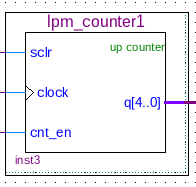
\includegraphics[scale=1]{./ct.png}
    \caption{5-разрядный счётчик в САПР Quartus II.}
    \label{fig:ct}
  \end{center}
\end{figure}

\begin{figure}
  \begin{center}
    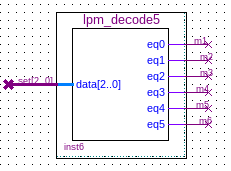
\includegraphics[scale=1]{./dc.png}
    \caption{8-разрядный дешифратор (используются только первые шесть разрядов) в САПР Quartus II.}
    \label{fig:dc}
  \end{center}
\end{figure}

\begin{figure}
  \begin{center}
    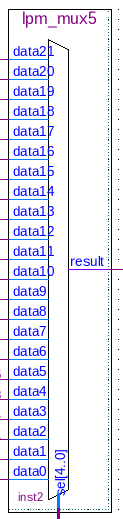
\includegraphics[scale=0.6]{./mux.png}
    \caption{32-разрядный мультиплексер (используются только первые 22 разряда) в САПР Quartus II.}
    \label{fig:mux}
  \end{center}
\end{figure}